%Este trabalho está licenciado sob a Licença Atribuição-CompartilhaIgual 4.0 Internacional Creative Commons. Para visualizar uma cópia desta licença, visite http://creativecommons.org/licenses/by-sa/4.0/deed.pt_BR ou mande uma carta para Creative Commons, PO Box 1866, Mountain View, CA 94042, USA.

\chapter{Produto vetorial}\label{cap_prodvec}
\thispagestyle{fancy}

De agora em diante, vamos trabalhar com um base ortonormal $B = (\vec{i}, \vec{j}, \vec{k})$ dita com orientação positiva, i.e. os vetores $\vec{i} = \overrightarrow{OI}$, $\vec{j} = \overrightarrow{OJ}$ e $\vec{k}=\overrightarrow{OK}$ estão dispostos em sentido anti-horário, veja Figura \ref{fig:base_pos}.

\begin{figure}[H]
  \centering
  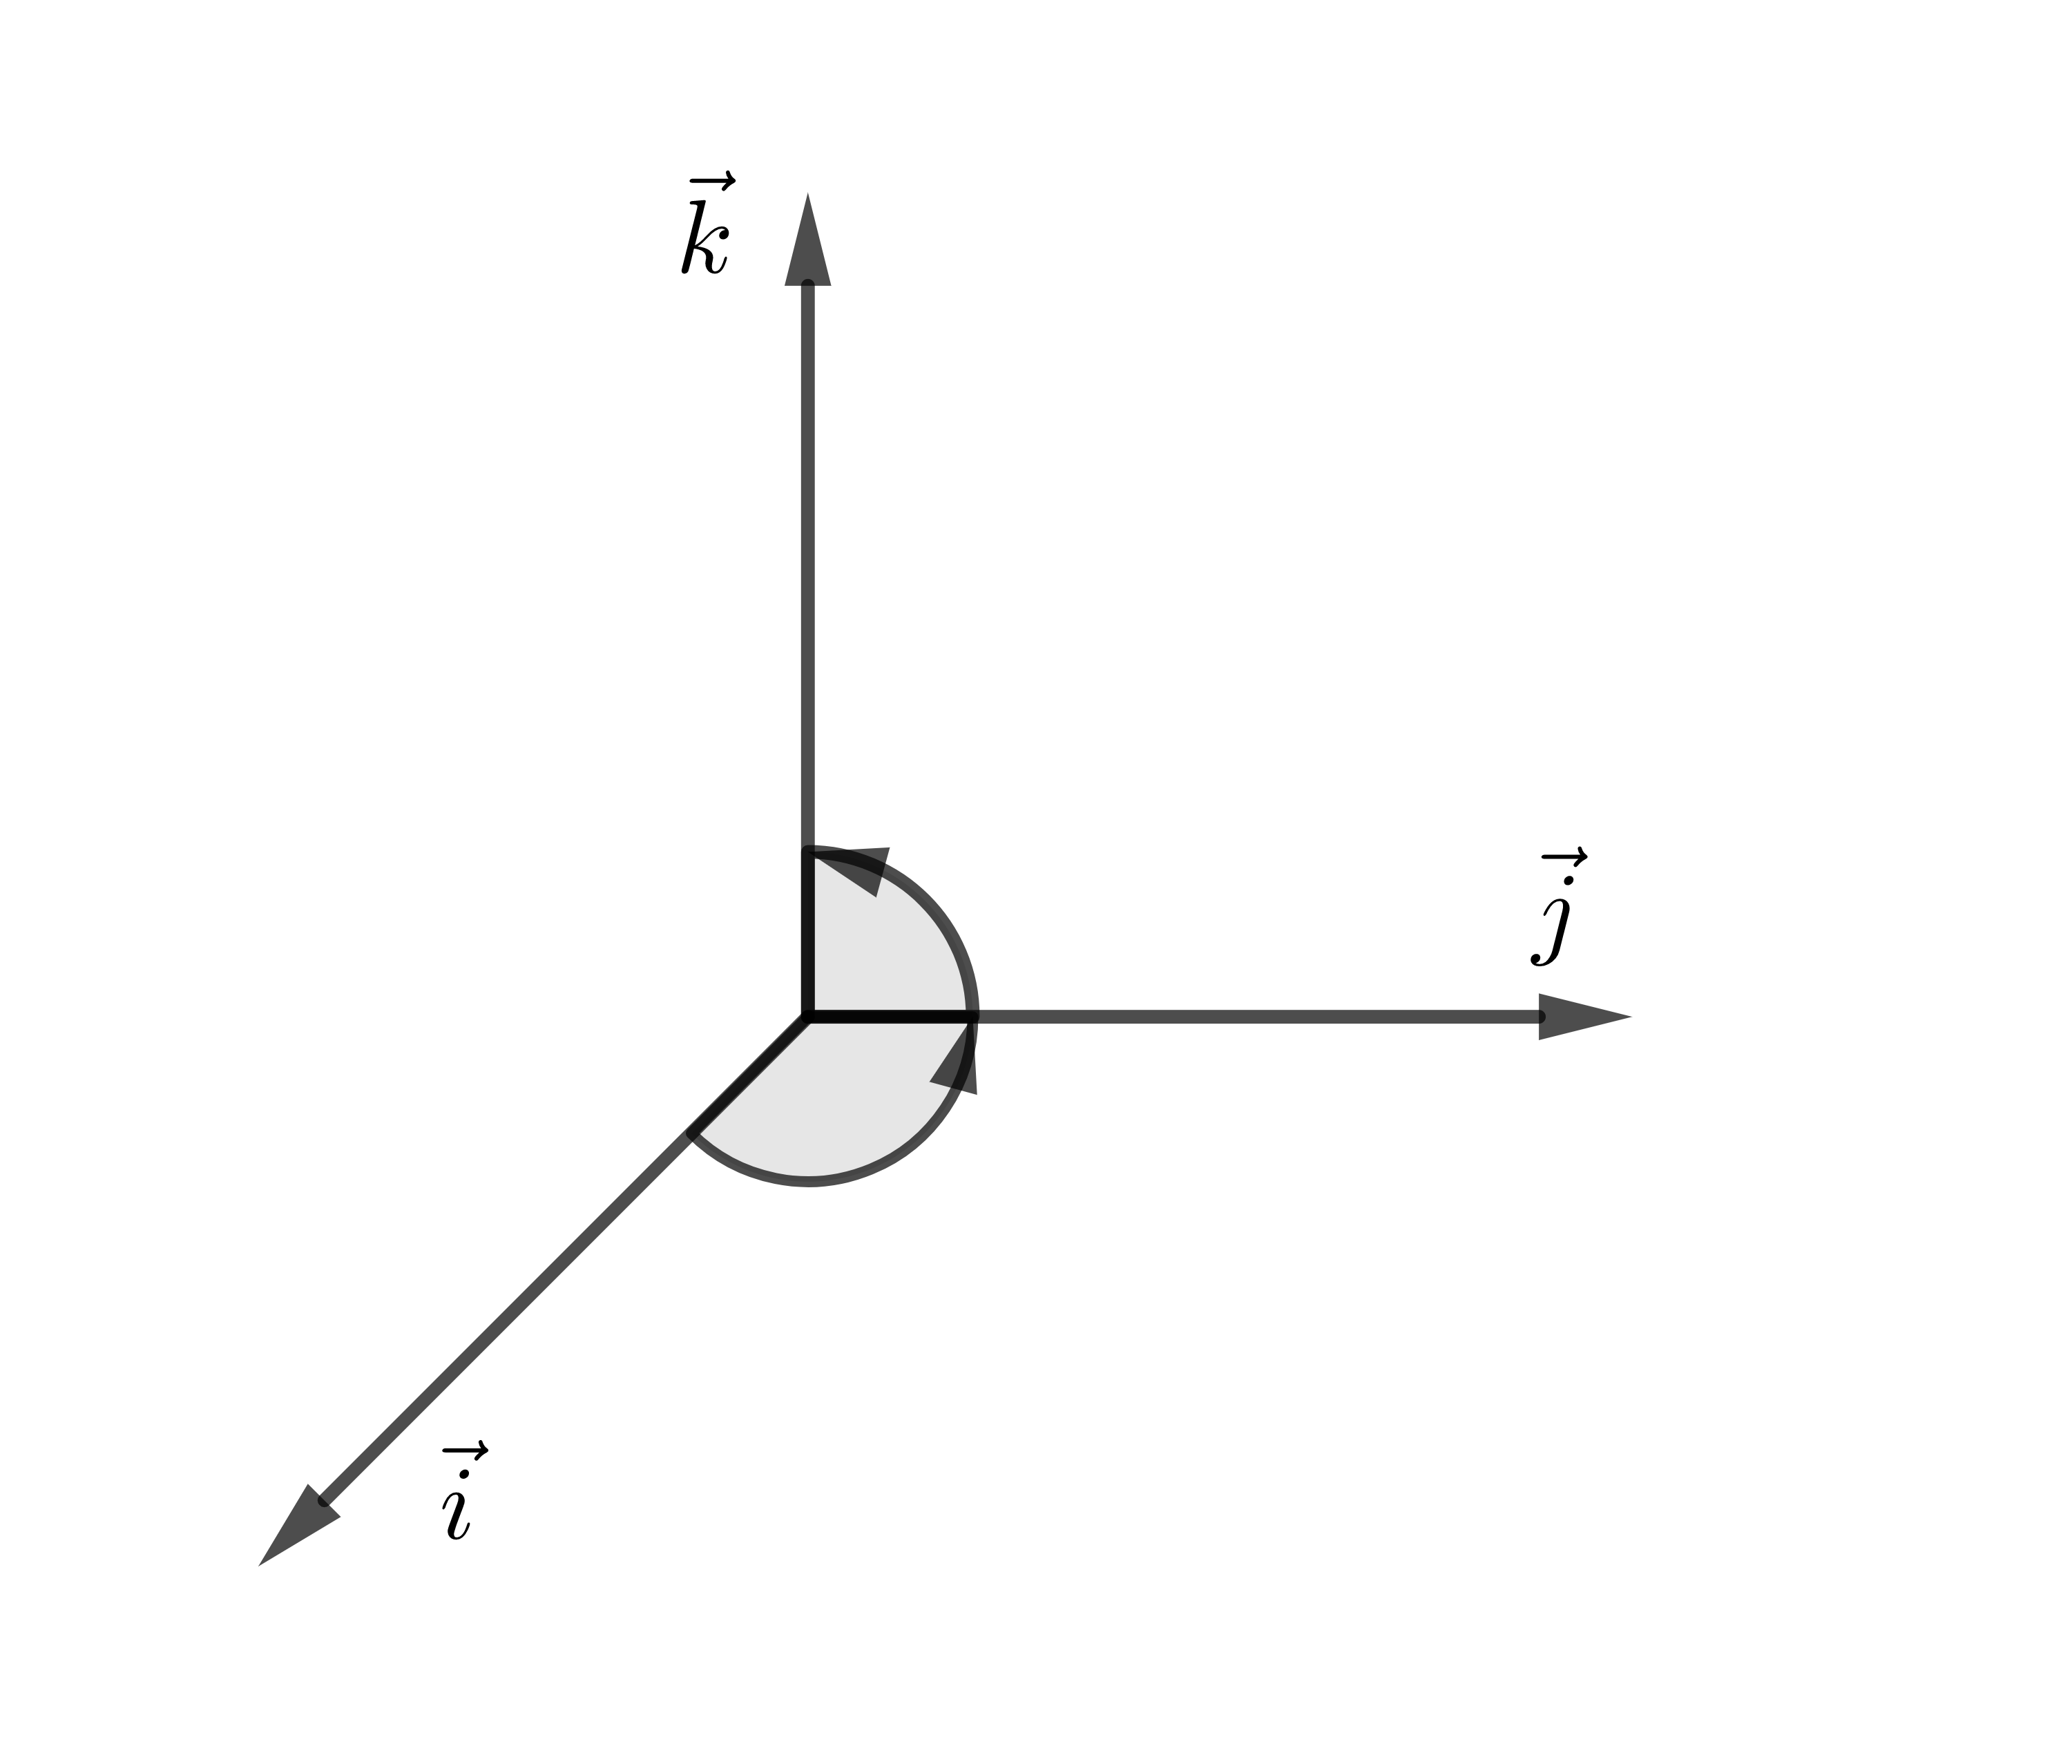
\includegraphics[width=0.7\textwidth]{./cap_prodvec/dados/fig_base_pos/fig_base_pos}
  \caption{Base ortonormal positiva.}
  \label{fig:base_pos}
\end{figure}

\section{Definição}\label{cap_prodvec_sec_prodvec}

Dados vetores $\vec{u}$ e $\vec{v}$, definimos o produto vetorial de $\vec{u}$ com $\vec{v}$, denotado por $\vec{u}\land\vec{v}$, como o vetor:
\begin{itemize}
\item se $\vec{u}$ e $\vec{v}$ são l.d., então $\vec{u}\land\vec{v} = \vec{0}$.
\item se $\vec{u}$ e $\vec{v}$ são l.i., então
  \begin{itemize}
  \item $|\vec{u}\land\vec{v}| = |\vec{u}||\vec{v}|\sen\alpha$, onde $\alpha$ é o ângulo entre $\vec{u}$ e $\vec{v}$,
  \item $\vec{u}\land\vec{v}$ é ortogonal a $\vec{u}$ e $\vec{v}$, e
  \item $\vec{u}$, $\vec{v}$ e $\vec{u}\land\vec{v}$ formam uma base positiva.
  \end{itemize}
\end{itemize}

\subsection{Interpretação geométrica}

Sejam dados $\vec{u}$ e $\vec{v}$ l.i.. Estes vetores determinam um paralelogramo, veja Figura \ref{fig:prodvec_interp}. Seja, então, $h$ a altura deste paralelogramo tendo $\vec{u}$ como sua base. Logo, a área do paralelogramo é o produto do comprimento da base com sua altura, neste caso
\begin{equation}
  |\vec{u}|h = |\vec{u}||\vec{v}|\sen\alpha.
\end{equation}
Ou seja, o produto vetorial $\vec{u}\land\vec{v}$ tem norma igual à área do paralelogramo determinado por $\vec{u}$ e $\vec{v}$.

\begin{figure}[H]
  \centering
  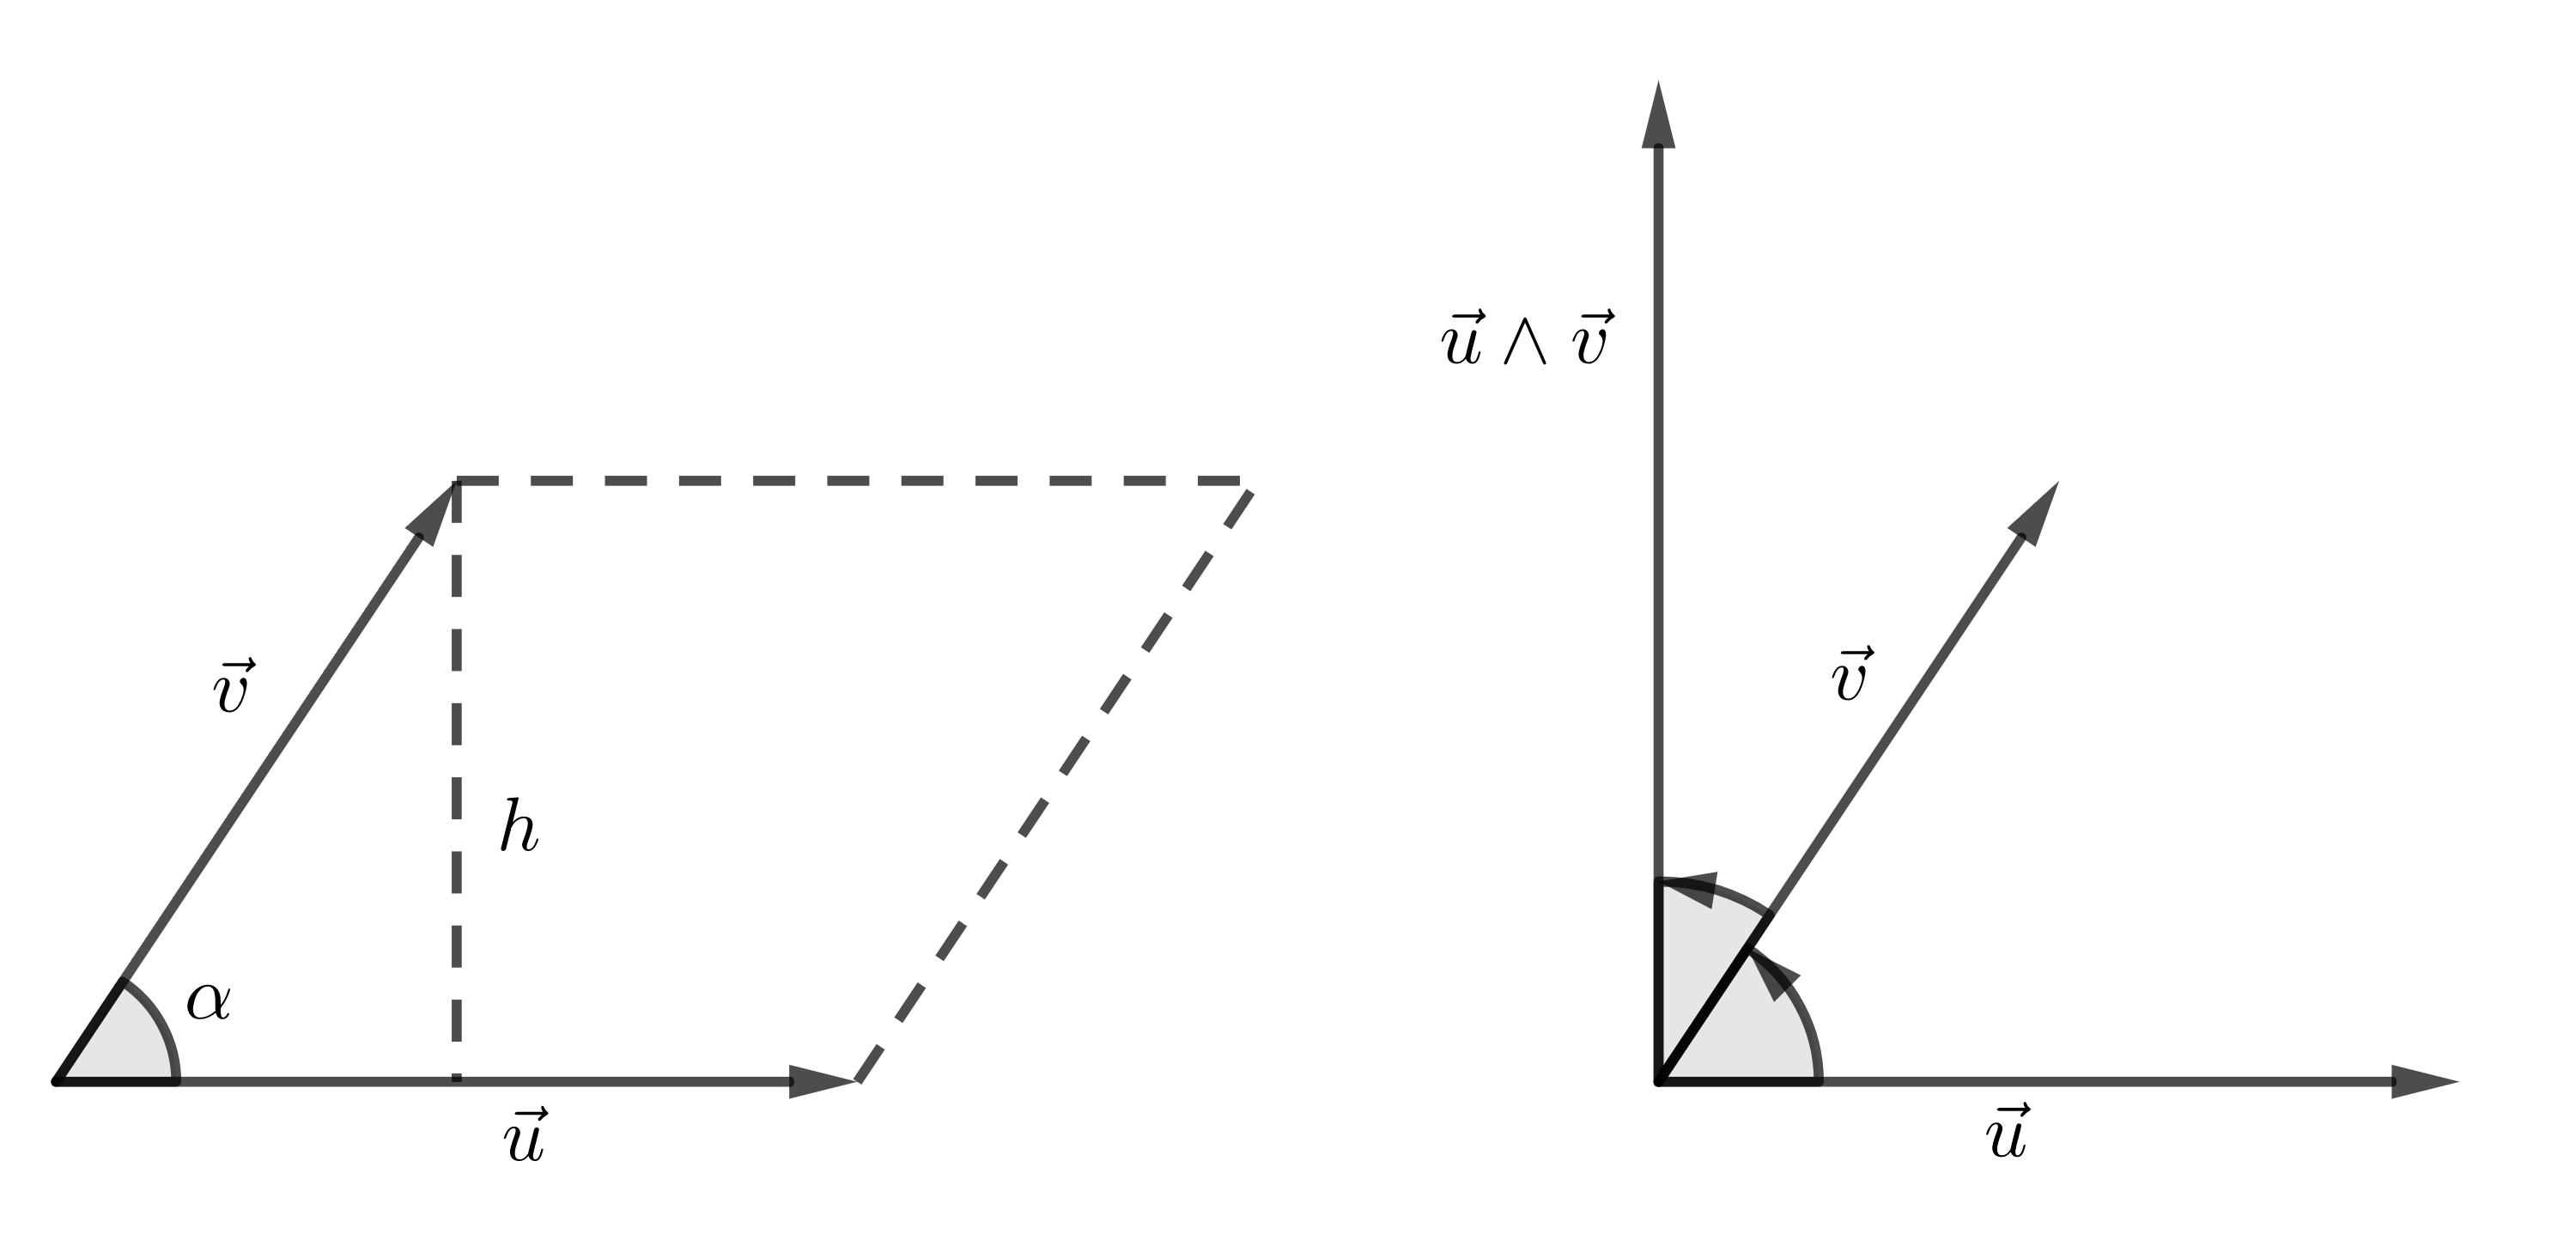
\includegraphics[width=0.7\textwidth]{./cap_prodvec/dados/fig_prodvec_interp/fig_prodvec_interp}
  \caption{Base ortonormal positiva.}
  \label{fig:base_pos}
\end{figure}

\subsection{Produto vetorial via coordenadas}\label{cap_prodvec_sec_coord}

Dados $\vec{u} = (u_1,u_2,u_3)$ e $\vec{v} = (v_1,v_2,v_3)$ em uma base ortonormal positiva, então
\begin{equation}
  \vec{u}\land\vec{v} =
  \begin{vmatrix}
    u_2 & u_3\\
    v_2 & v_3
  \end{vmatrix}\vec{i} -
  \begin{vmatrix}
    u_1 & u_3\\
    v_1 & v_3
  \end{vmatrix}\vec{j} +
  \begin{vmatrix}
    u_1 & u_2 \\
    v_1 & v_2
  \end{vmatrix}\vec{k}.
\end{equation}

\begin{obs}
  Uma regra mnemônica, é
  \begin{equation}
    \vec{u}\land\vec{v} =
    \begin{vmatrix}
      \vec{i} & \vec{j} & \vec{k} \\
      u_1 & u_2 & u_3 \\
      v_1 & v_2 & v_3
    \end{vmatrix}.
  \end{equation}
\end{obs}

\begin{ex}
  Dados os vetores $\vec{u} = (1,-2,1)$ e $\vec{v} = (0,2,-1)$, temos
  \begin{align}
    \vec{u}\land\vec{v} &=
                          \begin{vmatrix}
                            \vec{i} & \vec{j} & \vec{k} \\
                            u_1 & u_2 & u_3 \\
                            v_1 & v_2 & v_3
                          \end{vmatrix} \\
                        &=
                          \begin{vmatrix}
                            \vec{i} & \vec{j} & \vec{k} \\
                            1       & -2      & 1 \\
                            0       & 2       & -1
                          \end{vmatrix} \\
                        &= 0\vec{i} + \vec{j} + 2\vec{k}\\
                        &= (0,1,2).
  \end{align}
\end{ex}

\subsection{Exercícios}

\emconstrucao